\subsection{Perchè Q-learning?}
E' importante sottolineare come, nella letteratura relativa all'ambito del reinforcement learning, si è soliti andare a lavorare con quattro funzioni, che permettono di specificare come l'agente cambia la propria policy in funzione dell'esperienza acquisita, come si vede nella figura ~\ref{fig:Policy_update}.
Ovviamente, l'obbiettivo dell'agente è quello di ottenere il reward massimo fintantoche continua ad eseguire l'azione per cui è stato concepito: potremmo quindi introdurre il concetto di \textit{discounted return} al tempo \textit{t} definibile come:

\begin{center}
	$G_t = R_{t+1} + \gamma R_{t+2}+ \gamma^2\bullet R_{t+3} + ...$
	\label{eq:discounted_return}
\end{center}

dove con il coefficiente $\gamma$ andiamo a definire la \textit{lungimiranza} dell'agente: infatti se $\gamma = 0$ l'agente risulta essere \textit{greedy}, cercando di massimizzare il reward immediato; invece, mantenendo $\gamma < 1$, l'agente risulta essere in grado di dare un peso più o meno maggiore ai reward successivi, garantendo comunque la convergenza della sommatoria ~\ref{eq:discounted_return}.

Questa funzione appena introdotta risulta essere necessaria per definire due funzioni molto importanti:
\begin{itemize}
	\item \textbf{Value of a state, given a policy: } $v_\pi(s)$ che rappresenta il reward totale che ci si aspetta se l'agente segue la policy $\pi$ dall'istante t fino a $\infty$;
	\item \textbf{Value of a state-action pair, given a policy: } $q_\pi(s,a)$ indica sempre il reward che cumulerò seguendo sempre la stessa policy $\pi$, dopo però aver eseguito, nell'istante $t$ una specifica azione $a$.
\end{itemize}

I valori ottimali di queste funzioni, per completezza, sono rappresentati con l'apice $^*$, mentre i valori stimati, che sono quelli con cui poi si va effettivamente a lavorare, sono indicati tramite le lettere maiuscole, come si può notare nella figura ~\ref{fig:ValueFunctions}.

\begin{figure}[!h]
	\centering
	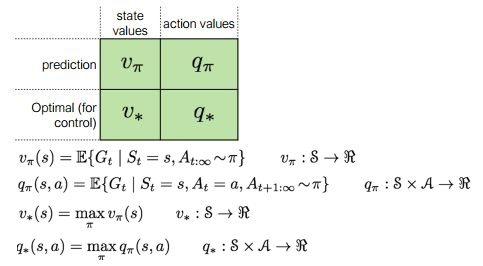
\includegraphics[width=0.5\textwidth]{Immagini/4_valueFunctions.JPG}
	\caption{4 value functions utilizzate per la policy update}
	\label{fig:ValueFunctions}
\end{figure}

Si può quindi facilmente intuire da dove deriva la nominazione di questo algoritmo: esso basa il proprio funzionamento sulla funzione \textit{Q}, la quale rappresenta la funzione cosidetta \textit{quality}, ovvero che indica quanto è utile una certa azione per aumentare il reward che si andrà ad ottenere nel futuro: si tratta inoltre di un algoritmo \textit{off-policy} poichè la funzione di q-learning apprende da azioni che stanno all'infuori delle policy corrente.
Essa può essere inserita in un quadro più generale di 4 funzioni, utilizzabili appunto dell'algoritmo di reinforcement learning per andare a gestire quella che è la policy dell'agente: esse sono riportate in figura ~\ref{fig:ValueFunctions}, con i rispettivi calcoli \textit{asintotici} necessari per ricavarne il valore.

Come evidenziato in precedenza, non possiamo però lavorare con i valori ottenibili tramite operatori di valore atteso, ma bensì risulta essere necessario andare ad utilizzare gli elementi stimati, ovvero rispettivamente $V_t(s)$ e $Q_t(s,a)$.

\subsection{Q-learning off policy control}
Il Q learning, come la maggior parte degli algoritmi di RL, va alla ricerca di un trade-off tra \textit{esploration e exploitation}: nel caso del Q learning si cerca, tramite un fattore di esplorazione (\textit{exploration rate}), di spingere l'algoritmo verso una scelta esplorativa piuttosto che di apprendimento, cercando di mantenere quindi una politica maggiormente esplorativa all'inizio del training per poi spostare l'attenzione sul fattore di apprendimento.
Il fatto che si tratti di un algoritmo off policy richiede in ingresso parametri aggiuntivi oltre a quelli forniti dall'ambiente (dimensione dello stato, numero di azioni...).
Tre sono i parametri aggiuntivi: $\alpha,\epsilon,\gamma$ che rappresentano rispettivamente 
\begin{itemize}
	\item learning rate: determina con quale estensione le nuove informazioni acquisite sovrascriveranno le vecchie informazioni; un fattore 0 impedirebbe all'agente di apprendere, al contrario un fattore 1 farebbe si che l'agente si interessi solo delle informazioni recenti
	\item exploration rate
	\item discounting rate: dovrebbe essere l'unico fattore non soggetto a decadimento, dato che esso determina l'importanza delle ricompense future, bilanciando reward immediato e futuro. Un fattore pari a 0 renderà l'agente opportunista, facendo si che consideri solo le ricompense attuali, mentre un fattore tendente ad 1 renderà l'agente attento anche alle ricompense che riceverà in futuro a lungo termine.
\end{itemize}
Per semplificare la trattazione, in questo contesto si è deciso di non considerare il decadimento dei parametri.

\begin{figure}[!h]
	\centering
	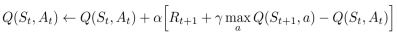
\includegraphics[width=0.5\textwidth]{Immagini/Q_estimation.JPG}
	\caption{Equazione di \textit{Bellman} utilizzata per andare ad aggiornare i valori della funzione Q}
	\label{fig:Q_estimation}
\end{figure}

Questa formula per l'update è stata implementata direttamente nel codice (come si vede in figura ~\ref{fig:Q_update}) all'interno dell'algoritmo ~\ref{alg:Q_policy}: in particolare è da evidenziare come il pedice $t$ applicato allo \textit{state} e \textit{action} rappresenta la condizione attuale; il pedice $t+1$ applicato allo stato, vuole invece rappresentare lo stato successivo che si raggiunge eseguendo l'azione A all'istante $t$.

\begin{figure}[!h]
	\centering
	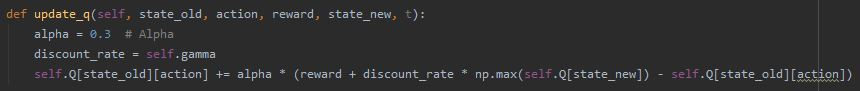
\includegraphics[width=0.5\textwidth]{Immagini/Q_update.JPG}
	\caption{Aggiornamento Q table}
	\label{fig:Q_update}
\end{figure}

\begin{algorithm}
		\SetAlgoLined
		\KwData{Parametri dell'algoritmo: step size $\alpha$ (con $0<=\alpha<=1$), $\epsilon>0$}
		\While{non sono terminati gli episodi:}{
			Inizializza lo stato S
			
			
			\While{non sono terminati gli step:}{
				Scegli azione A usando la policy derivata da Q (per esempio epsilon-greedy)
				
				
				Esegui l'azione A, osservando il reward (R) ottenuto e il nuovo stato (S') raggiunto
				
				
				Aggiorna Q(S,A) secondo la formula ~\ref{fig:Q_estimation}
				
				
				$S \leftarrow S'$ 
				
				
				Continua fino a che non si raggiunge uno stato terminare
			}
		}
		\caption{Q learning per la stima della policy $\pi$}
		\label{alg:Q_policy}
\end{algorithm}

\subsection{Scelta dell'azione e Q table}
Il metodo \textit{choose action} mostrato in figura ~\ref{fig:ChooseAction_Bucket}, permette la scelta dell'azione da intraprendere sulla base del trade off illustrato precedentemente tra esplorazione e apprendimento: si va infatti a scegliere la policy greedy che consiste in una scelta randomica dell'azione, oppure viene utilizzata la target policy a cui corrisponde il valore maggiore nella tabella stato-azione.
Si capisce quindi come Q-learning (in genere) sia in grado di andare a tener conto del problema di avere un trade-off tra:
\begin{itemize}
	\item \textbf{Exploiting: }scegliendo l'azione basata sul massimo valore della specifica azione, l'agente continua a rimanere fissato in quel punto, sfruttando al massimo il reward ottenibile, senza cercare eventuali altri stati in grado di fornire maggior reward;
	\item \textbf{Exploring: }selezionando randomicamente un'azione, rendiamo l'agente in grado di esplorare e scoprire nuovi stati, che altrimenti non avrebbe mai esplorato. 
\end{itemize}
\begin{figure}[!h]
	\centering
	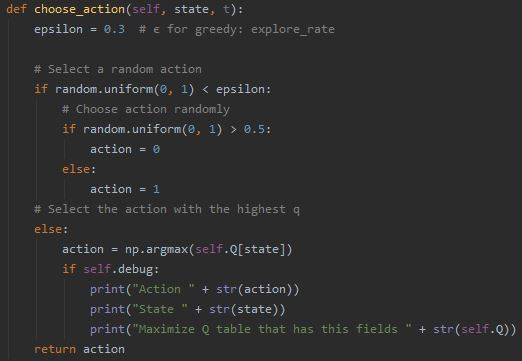
\includegraphics[width=0.5\textwidth]{Immagini/ChooseAction_QTable.JPG}
	\caption{Metodo per la stima della azione da eseguire}
	\label{fig:ChooseAction_Bucket}
\end{figure}

In particolare risulta quindi essere necessario spostarsi da uno spazio degli stati continuo ad uno discreto, con un numero finito e preferibilmente piccolo di stati discreti: infatti, meno stati abbiamo, più piccola risulterà essere la Q-table, e meno step l'agente dovrà eseguire per apprendere correttamente i valori che compongono la tabella. 

Tuttavia, pochi stati, potrebbero non essere sufficienti per rappresentare l'ambiente: nella nostra implementazione si è deciso di andare a discretizzare solamente 2 delle 4 variabili di stato, ovvero l'angolo $\theta$ e la velocità angolare $\theta'$ della barra; per quanto riguarda invece la posizione e la velocità del carrello, non discretizzandole, le si va a mappare come dei singoli valori scalari. La motivazione è il fatto che la probabilità del carrello di lasciare l'ambiente a destra o a sinistra e molto bassa, dando quindi maggior peso alla riduzione della dimensionalità.
Questa discretizzazione degli stati si traduce, a lato pratico, in una matrice con una struttura particolare, la quale dipende dal numero di bucket che si stanno utilizzando: supponiamo di aver settato, all'interno del nostro script Python, un vettore $buckets=(1, 1, 4, 5,)$: la Q-table risultante da questa discretizzazione è quella rappresentata in figura ~\ref{fig:Q_table_example} in cui si può vedere come, per ogni discretizzazione dell'angolo corrisponde un nuovo blocco di un numero di righe pari alla discretizzazione richiesta invece per la velcoità angolare. All'interno di ogni singola riga troviamo due differenti valori, i quali rappresentano appunto i Q-values relativi alle due possibili azioni eseguibili in ogni diverso stato.

\begin{figure}[!h]
	\centering
	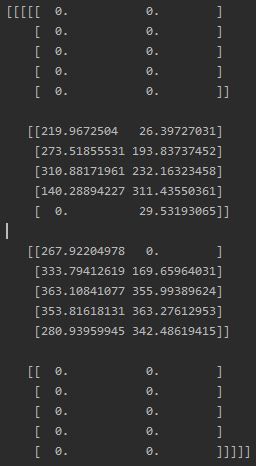
\includegraphics[width=0.2\textwidth]{Immagini/Example_of_Q_table.JPG}
	\caption{Possibile struttura della Q-table}
	\label{fig:Q_table_example}
\end{figure}

\subsection{Result}
La figura ~\ref{fig:QLearning_result} riportà l'andamento del reward in fase di training. L'algoritmo si considera risolto quando completa con successo 195 episodi consecutivi (sui 200 massimi disponibili): si nota infatti come nel grafico tutti gli ultimi total reward registrati siano sopra la soglia di vincita dell'algoritmo (linea verde).
L'andamento espresso dalla linea rossa invece indica un valore più \textit{smooth} del reward.

\begin{figure}[!h]
	\centering
	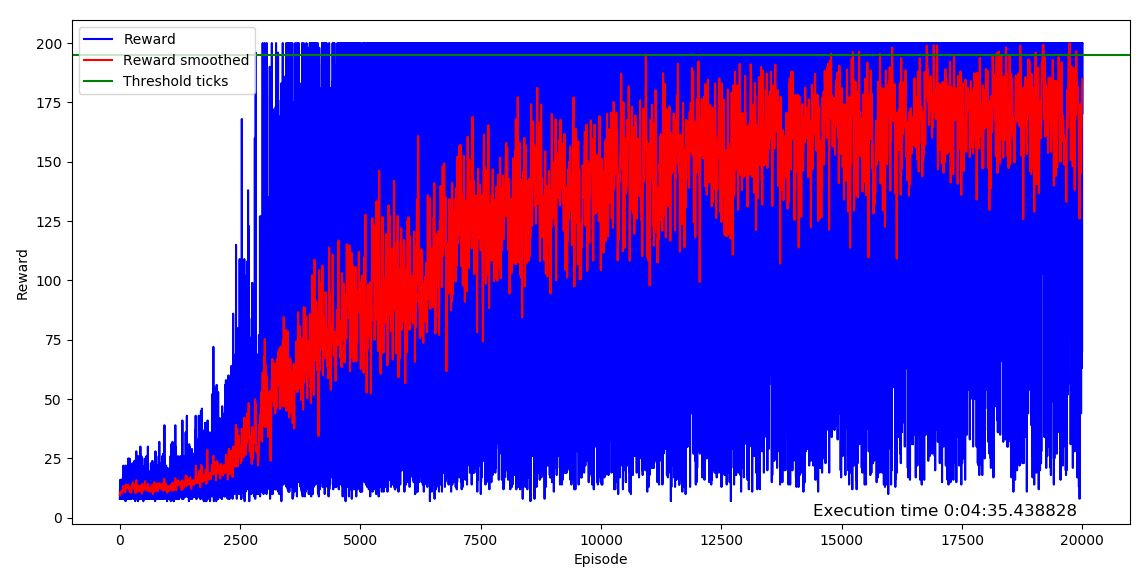
\includegraphics[width=0.8\textwidth]{Immagini/reward_20K.JPG}
	\caption{Andamento del Q learning}
	\label{fig:QLearning_result}
\end{figure}

Per andare a realizzare un confronto tra i diversi algoritmi, si è runnato l'agoritmo di Q-learning a bucket con un batch di 2000 iterazioni, ognuna delle  quali aveva una \textit{time threshold} di 200 iterazioni: come si può vedere in figura ~\ref{fig:QLearning_poor_result} il limite di iterazioni minime in cui il pole viene mantenuto in equilibrio non viene raggiunto. Si può notare anzi come l'agente non venga \textit{trainato} a sufficienza, raggiungendo prestazioni molto basse, rispetto ai successivi algoritmi.

\begin{figure}[!h]
	\centering
	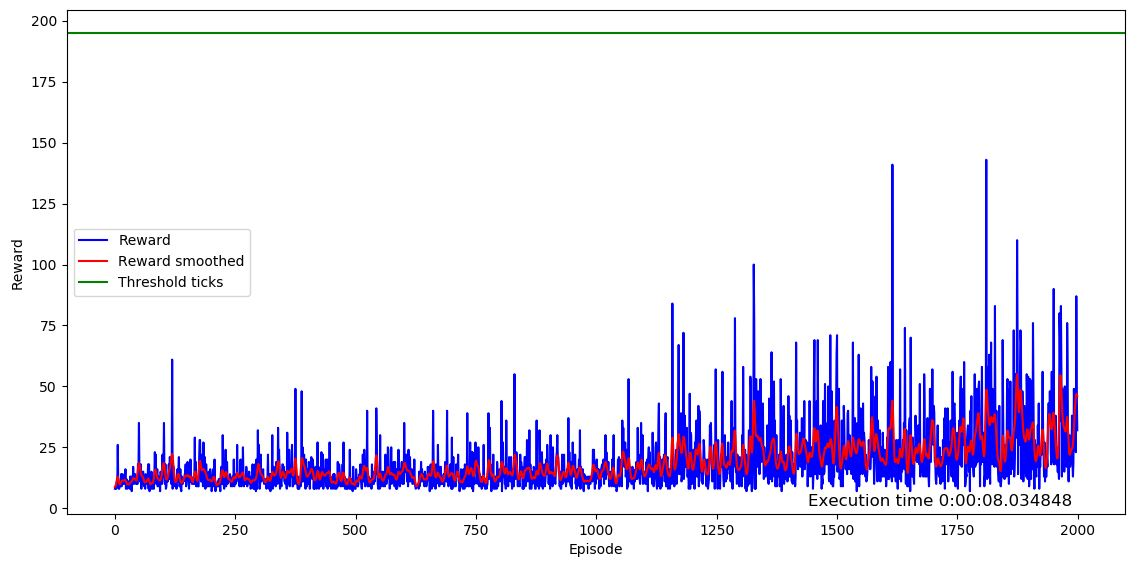
\includegraphics[width=0.8\textwidth]{Immagini/reward_2K.JPG}
	\caption{Andamento del Q learning confrontabile con atri algoritmi implementati}
	\label{fig:QLearning_poor_result}
\end{figure}

\newpage

